In this chapter, we describe augmenting encoders with the kind of background
knowledge that is available in external knowledge sources.

The model shown here is one specific kind of knowledge augmented encoder. It is an
ontology-aware recurrent neural network, an encoder that computes token level 
word representations grounded in an ontology (Wordnet).
The kind of background knowledge we deal with here is that of various senses of
words, and the generalizations of the concepts that correspond to each sense.
We encode that information by using Wordnet to find the 
collection of semantic concepts manifested by a word type, and represent a word 
type as a collection of concept embeddings. We show
how to integrate the proposed ontology-aware lexical representation with 
recurrent neural networks (RNNs) to model token sequences.

\section{Ontology-Aware Token Embeddings}
\paragraph{Types vs. Tokens} In accordance with standard terminology, we make
the following distinction 
between types and tokens in this chapter: By word types, we mean the surface form 
of the word, whereas by tokens we mean the instantiation of the surface form in 
a context. For example, the same word type \textit{`pool'} occurs as two 
different tokens in the sentences \textit{``He sat by the pool,''} and 
\textit{``He played a game of pool.''}

Type-level word embeddings map a word type (i.e., a surface form) to a dense 
vector of real numbers such that similar word types have similar embeddings. 
When pre-trained on a large corpus of unlabeled text, they provide an effective 
mechanism for generalizing statistical models to words which do not appear in 
the labeled training data for a downstream task. Most word embedding models 
define a single vector for each word type. However, a 
fundamental flaw in this design is their inability to distinguish between 
different meanings and abstractions of the same word. In the two sentences shown 
above, the word \textit{`pool'} has different meanings, but the same 
representation is typically used for both of them. Similarly, the fact that 
\textit{`pool'} and \textit{`lake'} are both kinds of water bodies is not 
explicitly incorporated in most type-level embeddings.
Furthermore, it has become a standard practice to tune pre-trained word 
embeddings as model parameters during training for an NLP task 
\cite[e.g.,][]{chen:14,lample:16}, potentially allowing the parameters of a 
frequent word in the labeled training data to drift away from related but rare 
words in the embedding space. 

In this chapter, we represent a word token in a given context by estimating a 
context-sensitive probability distribution over relevant concepts in WordNet 
\citep{miller1995wordnet} and use the expected value (i.e., weighted sum) of the 
concept embeddings as the token representation.
Effectively, we map each word type to a grid of concept embeddings (see 
Fig.~\ref{fig:ontolstm_tensor}), which are shared across many words. The word 
representation is computed as a distribution over the concept embeddings from 
the word's grid. We show how these distributions can be 
learned conditioned on the context when the representations are plugged into 
RNNs.
Intuitively, commonsense knowledge encoded as WordNet relations could 
potentially help with language understanding tasks. 
but mapping tokens to entities in WordNet is a challenge. One needs to at least 
disambiguate the sense of the token before being able to use the relevant 
information. Similarly, not all the hypernyms defined by WordNet may be useful 
for the task at hand as some may be too general to be informative.
 
\begin{figure}[t]
\begin{center}
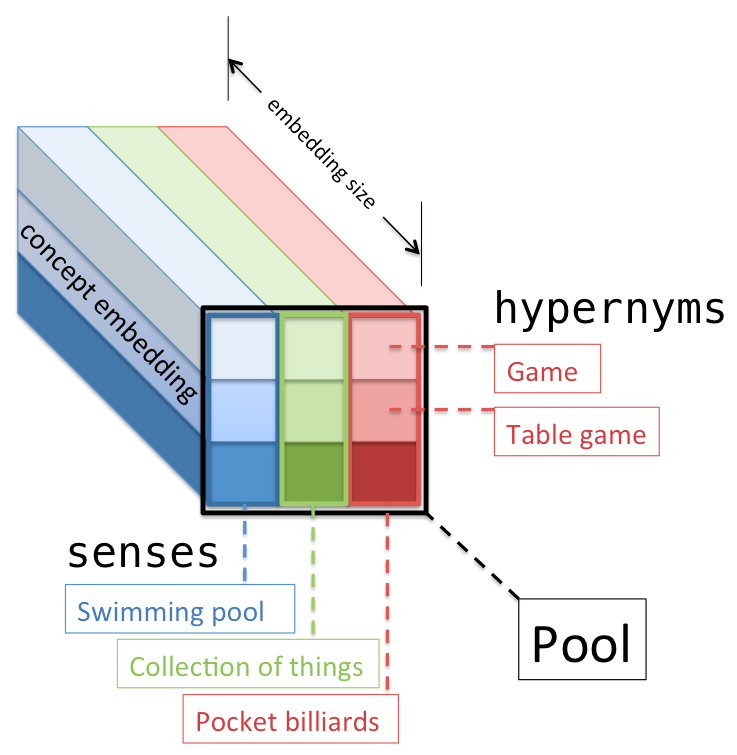
\includegraphics[width=3in]{figures/tensor2.png}
\caption{Example of ontology-aware lexical representation}
\label{fig:ontolstm_tensor}
\end{center}
\end{figure}

We take a task-centric approach towards doing this, and learn the token 
representations jointly with the task-specific parameters.
In addition to providing context-sensitive token embeddings, the proposed method 
implicitly regularizes the embeddings of related words by forcing related words 
to share similar concept embeddings. 
As a result, the representation of a rare word which does not appear in the 
training data for a downstream task benefits from all the updates to related 
words which share one or more concept embeddings. While the results presented in this thesis are from a model that relies on WordNet, 
and we exploit the order of senses given by WordNet, the approach is, in principle 
applicable to any ontology, with appropriate modifications. Here, we do not assume the inputs are 
sense tagged.

We evaluate the proposed embeddings in two applications. The first is predicting prepositional phrase 
(PP) attachments (see Section~\ref{sec:ontolstm_pp_model}), a challenging problem which 
emphasizes the selectional preferences between words in the PP and each of the 
candidate head words.  The second application is Textual Entailment (see Section~\ref{sec:ontolstm_snli}),
a task that benefits from hypernymy features from WordNet, providing generalization information.
Our empirical results and detailed analysis (see Section\ref{sec:ontolstm_pp_experiments} and Section~\ref{sec:ontolstm_pp_experiments}) show 
that the proposed embeddings effectively use WordNet to improve the accuracy of 
PP attachment predictions.

\section{Related Work}
\label{sec:ontolstm_related_work}
% concept embeddings
This work is related to various lines of research within the NLP community: dealing with synonymy and homonymy in word representations both in the context of distributed embeddings and more traditional vector spaces; hybrid models of distributional and knowledge based semantics; and selectional preferences and their relation with syntactic and semantic relations.

\subsection{Multi-prototype Word Vectors}
The need for going beyond a single vector per word-type has been well established for a while, and many efforts were focused on building multi-prototype vector space models of meaning \cite[][etc.]{reisinger2010multi,huang2012improving,chen2014unified,jauhar:15,neelakantan2015efficient,arora2016linear}. However, the target of all these approaches is obtaining multi-sense word vector spaces, either by incorporating sense tagged information or other kinds of external context. The number of vectors learned is still fixed, based on the preset number of senses. In contrast, our focus is on learning a context dependent distribution over those concept representations. Other work not necessarily related to multi-sense vectors, but still related to our work includes \cite{belanger:15}'s work which proposed a Gaussian linear dynamical system for estimating token-level word embeddings, and \cite{Vilnis2014WordRV}'s work which proposed mapping each word type to a density instead of a point in a space to account for uncertainty in meaning. These approaches do not make use of lexical ontologies and are not amenable for joint training with a downstream NLP task. 

Related to the idea of concept embeddings is \cite{rothe:15} who estimated WordNet synset representations, given pre-trained type-level word embeddings.
In contrast, our work focuses on estimating token-level word embeddings as context sensitive distributions of concept embeddings.

\subsection{Hybrid Models of Knowledge-based and Distributional Semantics}
There is a large body of work that tried to improve word embeddings using external resources. \cite{yu:14} extended the CBOW model \cite{mikolov:13} by adding an extra term in the training objective for generating words conditioned on similar words according to a lexicon.
\cite{jauhar:15} extended the skipgram model \cite{mikolov:13} by representing word senses as latent variables in the generation process, and used a structured prior based on the ontology.
\cite{faruqui:15} used belief propagation to update pre-trained word embeddings on a graph that encodes lexical relationships in the ontology.
Similarly, \cite{johansson2015embedding} improved word embeddings by representing each sense of the word in a way that reflects the topology of the semantic network they belong to, and then representing the words as convex combinations of their senses.
In contrast to previous work that was aimed at improving \textit{type level} word representations, we propose an approach for obtaining \textit{context-sensitive} embeddings at the \textit{token level}, while jointly optimizing the model parameters for the NLP task of interest.

\subsection{WordNet as a source for Selectional Preferences}
\cite{resnik:93} showed the applicability of semantic classes and selectional preferences to resolving syntactic ambiguity. \cite{Zapirain2013SelectionalPF} applied models of selectional preferences automatically learned from WordNet and distributional information, to the problem of semantic role labeling. \cite{resnik:93,brill1994rule,agirre2008improving} and others have used WordNet information towards improving prepositional phrase attachment predictions.

\section{WordNet-Grounded Context-Sensitive Token Embeddings}
\label{sec:ontolstm_input_rep}

In this section, we focus on defining our context-sensitive token embeddings. 
We first describe our grounding of word types using WordNet concepts.
Then, we describe our model of context-sensitive token-level embeddings as a weighted sum of WordNet concept embeddings. 

\subsection{WordNet Grounding}
We use WordNet to map each word type to a set of synsets, including possible generalizations or abstractions. 
Among the labeled relations defined in WordNet between different synsets, we focus on the hypernymy relation to help model generalization and selectional preferences between words, which is especially important for predicting PP attachments \citep{resnik:93}.
To ground a word type, we identify the set of (direct and indirect) hypernyms of the WordNet senses of that word.
A simplified grounding of the word `pool' is illustrated in Figure \ref{fig:ontolstm_wordnet_grounding}.
This grounding is key to our model of token embeddings, to be described in the following subsections. 

\subsection{Context-Sensitive Token Embeddings}
\label{sec:ontolstm_embedding_model}

Our goal is to define a context-sensitive model of token embeddings which can be used as a drop-in replacement for traditional type-level word embeddings.

\paragraph{Notation.}
Let $\textit{Senses}(w)$ be the list of synsets defined as possible word senses of a given \underline{w}ord type $w$ in WordNet, and $\textit{Hypernyms}(s)$ be the list of hypernyms for a \underline{s}ynset $s$.
\footnote{For notational convenience, we assume that $s \in \textit{Hypernyms}(s)$.} Figure~\ref{fig:ontolstm_wordnet_grounding} shows an example. In the figure, solid arrows
represent possible senses and dashed arrows represent hypernym relations. Note that the same set of concepts are used to ground the word \textit{`pool'} regardless of its context.
Other WordNet senses for \textit{`pool'} were removed from the figure for simplicity. According to figure, 
\begin{align}
\textit{Senses}&(\text{pool}) = [\text{pond.n.01, pool.n.09}], \text{and} \nonumber \\
\textit{Hypernyms}&(\text{pond.n.01}) = [\text{pond.n.01, lake.n.01}, \nonumber \\
&\text{body\_of\_water.n.01, entity.n.01}] \nonumber
\end{align}

\begin{figure}
\begin{center}
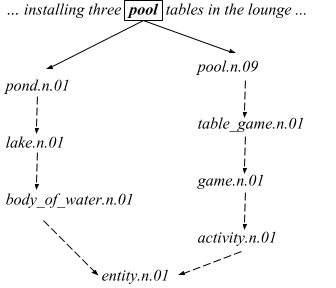
\includegraphics[width=3in]{figures/ontolstm_wordnet_grounding.png}
\caption{An example grounding for the word \textit{pool}}
\label{fig:ontolstm_wordnet_grounding}
\end{center}
\end{figure}
Each WordNet synset $s$ is associated with a set of parameters $\mathbf{v}_s \in \mathbb{R}^n$ which represent its embedding. 
This parameterization is similar to that of \cite{rothe:15}.

\paragraph{Embedding model.}

\begin{figure}[t]
\begin{center}
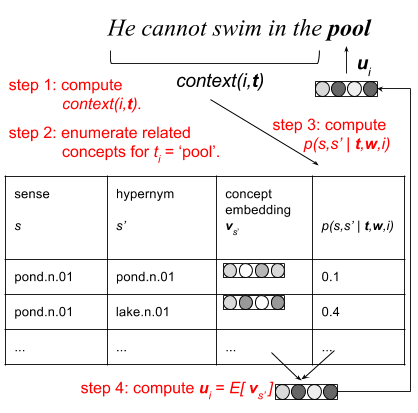
\includegraphics[width=3.5in]{figures/ontolstm_token_embedding.png}
\caption{Steps for computing the context-sensitive token embedding for the word \textit{`pool'}, as described in Section\ref{sec:ontolstm_embedding_model}.
\label{fig:ontolstm_token_embedding}}
\end{center}
\end{figure}

Given a sequence of \underline{t}okens $\boldsymbol{t}$ and their corresponding word types $\boldsymbol{w}$, let $\mathbf{u}_i  \in \mathbb{R}^n$
be the embedding of the word token $t_i$ at position $i$. Unlike most embedding models, the token embeddings $\mathbf{u}_i$ are not parameters.
Rather, $\mathbf{u}_i$ is computed as the expected value of concept embeddings used to ground the word type $w_i$ corresponding to the token $t_i$:
\begin{align}
\mathbf{u}_i = \sum_{s \in \textit{Senses}(w_i)} 
\sum_{s' \in \textit{Hypernyms}(s)}
p(s, s' \mid \boldsymbol{t}, \boldsymbol{w}, i) \  &\mathbf{v_{s'}} 
 \label{eq:ontolstm_token_embedding}\end{align}
such that
\begin{equation}
\sum_{s \in \textit{Senses}(w_i)} \sum_{s' \in \textit{Hypernyms}(s)} p(s, s' \mid \boldsymbol{t}, \boldsymbol{w}, i) = 1
\nonumber \end{equation}

The distribution which governs the expectation over synset embeddings factorizes into two components:
\begin{align}
p(s, s' \mid \boldsymbol{t}, \boldsymbol{w}, i) \propto& 
\lambda_{w_i} \exp^{-\lambda_{w_i} \  \textit{rank}(s, w_i)} \times \nonumber \\
&  \textit{MLP}( [\mathbf{v}_{s'}; \textit{context}(i, \boldsymbol{t})]) 
\label{eq:ontolstm_attention}
\end{align}
The first component, $\lambda_{w_i} \exp^{-\lambda_{w_i} \  \textit{rank}(s, w_i)}$, is a sense prior which reflects the prominence of each word sense for a given word type. Here, we exploit\footnote{Note that for ontologies where such information is not available, our method is still applicable but without this component.
We show the effect of using a uniform sense prior in Section~\ref{sec:ontolstm_pp_analysis}.} the fact that WordNet senses are ordered in descending order of their frequencies, obtained from sense tagged corpora, and parameterize the sense prior like an exponential distribution.
$rank(s, w_i)$ denotes the rank of sense $s$ for the word type $w_i$, thus $rank(s, w_i)=0$ corresponds to $s$ being the first sense of $w_i$.
The scalar parameter ($\lambda_{w_i}$) controls the decay of the probability mass, which is learned along with the other parameters in the model. Note that sense priors are defined for each word type ($w_i$), and are shared across all tokens which have the same word type.

$\textit{MLP}( [\mathbf{v}_{s'}; \textit{context}(i, \boldsymbol{t})])$, the second component, is what makes the token representations context-sensitive. 
It scores each concept in the WordNet grounding of $w_i$ by feeding the concatenation of the concept embedding and a dense vector that summarizes the textual context into a multilayer perceptron ($\textit{MLP}$) with two $tanh$ layers followed by a $softmax$ layer.
This component is inspired by the soft attention often used in neural machine translation \citep{bahdanau:14}.\footnote{Although soft attention mechanism is typically used to explicitly represent the importance of each item in a sequence, it can also be applied to non-sequential items.} The definition of the $\textit{context}$ function is dependent on the encoder used to encode the context.
We describe a specific instantiations of this function in Section~\ref{sec:ontolstm_pp_model} and Section~\ref{sec:ontolstm_snli}.

To summarize, Figure \ref{fig:ontolstm_token_embedding} illustrates how to compute the embedding of a word token $t_i=\textit{`pool'}$ in a given context:
\begin{enumerate}
    \item compute a summary of the context $\textit{context}(i, \boldsymbol{t})$,
    \item enumerate related concepts for $t_i$,
    \item compute $p(s,s'\mid \boldsymbol{t}, \boldsymbol{w}, i)$ for each pair $(s,s')$, and
    \item compute $\mathbf{u}_i = \mathbb{E}[\mathbf{v}_{s'}]$.
\end{enumerate}

In the following section, we describe our model for predicting PP attachments, including our definition for $\textit{context}$ for this problem.

\section{PP Attachment}
\label{sec:ontolstm_pp_model}
Disambiguating PP attachments is an important and challenging NLP problem. Since modeling hypernymy and selectional preferences is critical for successful prediction of PP attachments \citep{resnik:93}, it is a good fit for evaluating our WordNet-grounded context-sensitive embeddings.

\begin{figure}[t]
\begin{center}
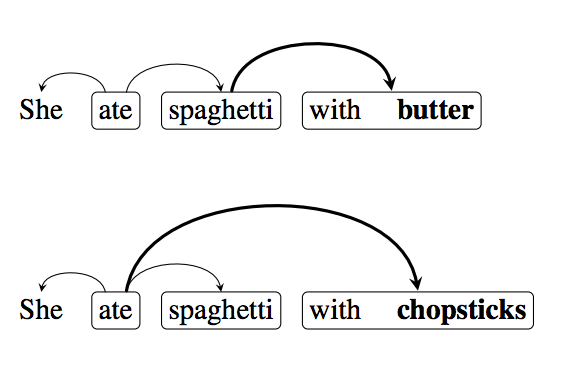
\includegraphics[width=3.2in]{figures/pp_attachment_example.png}
\label{fig:ontolstm_pp_example}
\caption{ Two sentences illustrating the importance
of lexicalization in PP attachment decisions.}
\end{center}
\end{figure}

Figure \ref{fig:ontolstm_pp_example}, reproduced from \cite{belinkov2014exploring}, illustrates an example of the PP attachment prediction problem.
In the top sentence, the PP \textit{`with butter'} attaches to the noun \textit{`spaghetti'}. 
In the bottom sentence, the PP \textit{`with chopsticks'} attaches to the verb \textit{`ate'}.
The accuracy of a competitive English dependency parser at predicting the head word of an ambiguous prepositional phrase is 88.5\%, significantly lower than the overall unlabeled attachment accuracy of the same parser (94.2\%).\footnote{See Table \ref{tab:ontolstm_parser_ppa_results} for detailed results.}

This section formally defines the problem of PP attachment disambiguation, describes our baseline model, then shows how to integrate the token-level embeddings in the model.

\subsection{Problem Definition}
\label{sec:ontolstm_pp_problem_definition}
We follow \cite{belinkov2014exploring}'s definition of the PP attachment problem.
Given a \underline{p}reposition $p$ and its direct \underline{d}ependent $d$ in the prepositional phrase (PP), our goal is to predict the correct head word for the PP among an ordered list of candidate \underline{h}ead words $\boldsymbol{h}$.
Each example in the train, validation, and test sets consists of an input tuple $\langle \boldsymbol{h}, p, d \rangle$ and an output index $k$ to identify the correct head among the candidates in $\boldsymbol{h}$. Note that the order of words that form each $\langle \boldsymbol{h}, p, d\rangle$ is the same as that in the corresponding original sentence.

\subsection{Model Definition}
Both our proposed and baseline models for PP attachment use bidirectional RNN with LSTM cells (bi-LSTM) to encode the sequence $\boldsymbol{t} = \langle h_1, \ldots, h_K, p, d \rangle$.

We score each candidate head by feeding the concatenation of the output bi-LSTM vectors for the head $h_k$, the preposition $p$ and the direct dependent $d$ through an MLP, with a fully connected $\textit{tanh}$ layer to obtain a non-linear projection of the concatenation, followed by a fully-connected $\textit{softmax}$ layer:

\begin{align}
p(h_k \text{is head}) = \textit{MLP}_{\textit{attach}}([&\textit{lstm\_out}(h_k);\nonumber \\
&\textit{lstm\_out}(p);\nonumber \\
&\textit{lstm\_out}(d)]) \label{eq:pp_model}
\end{align}
To train the model, we use cross-entropy loss at the output layer for each candidate head in the training set.
At test time, we predict the candidate head with the highest probability according to the model in Eq. \ref{eq:pp_model}, i.e.,
\begin{align}
\hat{k} = \arg\max_k p(h_k \text{is head} = 1).
\end{align}
This model is inspired by the Head-Prep-Child-Ternary model of \cite{belinkov2014exploring}. 
The main difference is that we replace the input features for each token with the output bi-RNN vectors.

We now describe the difference between the proposed and the baseline models. Generally, let $\textit{lstm\_in}(t_i)$ and $\textit{lstm\_out}(t_i)$ represent the input and output vectors of the bi-LSTM for each token $t_i \in \boldsymbol{t}$ in the sequence. The outputs at each timestep are obtained by concatenating those of the forward and backward LSTMs.

\paragraph{Baseline model.}
In the baseline model, we use type-level word embeddings to represent the input vector $\textit{lstm\_in}(t_i)$ for a token $t_i$ in the sequence. The word embedding parameters are initialized with pre-trained vectors, then tuned along with the parameters of the bi-LSTM and $\textit{MLP}_{\textit{attach}}$. We call this model \textbf{LSTM-PP}.

\paragraph{Proposed model.}
\label{sec:ontolstm_proposed_ppa_model}
In the proposed model, we use token level word embedding as described in Section\ref{sec:ontolstm_input_rep} as the input to the bi-LSTM, i.e., $\textit{lstm\_in}(t_i) = \mathbf{u}_i$. The context used for the attention component is simply the hidden state from the previous timestep. However, since we use a bi-LSTM, the model essentially has two RNNs, and accordingly we have two context vectors, and associated attentions. That is, $\textit{context}_f\textit{(i, \textbf{t})} = \textit{lstm\_in}(t_{i-1})$ for the forward RNN and $\textit{context}_b\textit{(i, \textbf{t})} = \textit{lstm\_in}(t_{i+1})$ for the backward RNN. Consequently, each token gets two representations, one from each RNN. The synset embedding parameters are initialized with pre-trained vectors and tuned along with the sense decay ($\lambda_{w}$) and MLP parameters from Eq. \ref{eq:ontolstm_attention}, the parameters of the bi-LSTM and those of $\textit{MLP}_{\textit{attach}}$. We call this model \textbf{OntoLSTM-PP}.

\subsection{Experiments}
\label{sec:ontolstm_pp_experiments} 

\paragraph{Dataset and evaluation.} We used the English PP attachment dataset created and made available by \cite{belinkov2014exploring}. The training and test splits contain 33,359 and 1951 labeled examples respectively. As explained in Section\ref{sec:ontolstm_pp_problem_definition}, the input for each example is 1) an ordered list of candidate head words, 2) the preposition, and 3) the direct dependent of the preposition.
The head words are either nouns or verbs and the dependent is always a noun. 
All examples in this dataset have at least two candidate head words.
As discussed in \cite{belinkov2014exploring}, this dataset is a more realistic PP attachment task than the RRR dataset \citep{ratnaparkhi1994maximum}.
The RRR dataset is a binary classification task with exactly two head word candidates in all examples.
The context for each example in the RRR dataset is also limited which defeats the purpose of our context-sensitive embeddings.

\paragraph{Model specifications and hyperparameters.} 
For efficient implementation, we use mini-batch updates with the same number of senses and hypernyms for all examples, padding zeros and truncating senses and hypernyms as needed.
For each word type, we use a maximum of $S$ senses and $H$ indirect hypernyms from WordNet.
In our initial experiments on a held-out development set (10\% of the training data), we found that values greater than $S=3$ and $H=5$ did not improve performance. We also used the development set to tune the number of layers in $\textit{MLP}_{\textit{attach}}$ separately for the \textit{OntoLSTM-PP} and \textit{LSTM-PP}, and the number of layers in the attention MLP in \textit{OntoLSTM-PP}.
When a synset has multiple hypernym paths, we use the shortest one. 
Finally, words types which do not appear in WordNet are assumed to have one unique sense per word type with no hypernyms. Since the POS tag for each word is included in the dataset, we exclude WordNet synsets which are incompatible with the POS tag.
The synset embedding parameters are initialized using the synset vectors obtained by running AutoExtend \citep{rothe:15} on 100-dimensional GloVe \citep{pennington2014glove} vectors for WordNet 3.1. We refer to this embedding as \textit{GloVe-extended}. Representation for the OOV word types in LSTM-PP and OOV synset types in \textit{OntoLSTM-PP} were randomly drawn from a uniform 100-d distribution. 
Initial sense prior parameters ($\lambda_w$) were also drawn from a uniform 1-d distribution.

\paragraph{Baselines.} In our experiments, we compare our proposed model, \textit{OntoLSTM-PP} with three baselines -- \textit{LSTM-PP} initialized with GloVe embedding, \textit{LSTM-PP} initialized with GloVe vectors retrofitted to WordNet using the approach of \cite{faruqui:15} (henceforth referred to as \textit{GloVe-retro}), and finally the best performing standalone PP attachment system from \cite{belinkov2014exploring}, referred to as \textit{HPCD (full)} in the paper. \textit{HPCD (full)} is a neural network model that learns to compose the vector representations of each of the candidate heads with those of the preposition and the dependent, and predict attachments. The input representations are enriched using syntactic context information, POS, WordNet and VerbNet \citep{kipper2008large} information and the distance of the head word from the PP is explicitly encoded in composition architecture. In contrast, we do not use syntactic context, VerbNet and distance information, and do not explicitly encode POS information.

\subsubsection{PP Attachment Results}
\begin{table}
    \centering
    \begin{tabular}{|l|c|c|c|c|}
    \hline
    \textbf{System} & \textbf{Initialization} & \textbf{Embedding} & \textbf{Resources} & \textbf{Test Acc.}\\
    \hline
    HPCD (full) & Syntactic-SG & Type & WordNet, VerbNet & 88.7 \\
    \hline
    LSTM-PP  & GloVe & Type & - & 84.3 \\
    LSTM-PP & GloVe-retro & Type & WordNet & 84.8 \\
    OntoLSTM-PP & GloVe-extended & Token & WordNet & \textbf{89.7} \\
    \hline
    \end{tabular}
    \caption{Prepositional Phrase Attachment Results with OntoLSTM}
    \label{tab:ontolstm_direct_ppa_results}
\end{table}
%We compare OntoLSTM-PP to two instantiations of LSTM-PP as well as the best performing .  In all systems, the word type embedding or synset embedding is tuned during training. 
Table \ref{tab:ontolstm_direct_ppa_results} shows that our proposed token level embedding scheme \textit{OntoLSTM-PP} outperforms the better variant of our baseline \textit{LSTM-PP} (with GloVe-retro intialization) by an absolute accuracy difference of 4.9\%, 
or a relative error reduction of 32\%.
\textit{OntoLSTM-PP} also outperforms \textit{HPCD (full)}, the previous best result on this dataset. \textit{HPCD (full)} is from the original paper, and it uses syntactic SkipGram. \textit{GloVe-retro} is GloVe vectors retrofitted \citep{faruqui:15} to WordNet 3.1, and \textit{GloVe-extended} refers to the synset embeddings obtained by running AutoExtend \citep{rothe:15} on GloVe.

Initializing the word embeddings with \textit{GloVe-retro} (which uses WordNet as described in \cite{faruqui:15}) instead of GloVe amounts to a small improvement, compared to the improvements obtained using \textit{OntoLSTM-PP}.
This result illustrates that our approach of dynamically choosing a context sensitive distribution over synsets is a more effective way of making use of WordNet.


\paragraph{Effect on dependency parsing.} Following \cite{belinkov2014exploring}, we used RBG parser \citep{lei2014low}, and modified it by adding a binary feature indicating the PP attachment predictions from our model. 

We compare four ways to compute the additional binary features: 1) the predictions of the best standalone system \textit{HPCD (full)} in \cite{belinkov2014exploring}, 2) the predictions of our baseline model \textit{LSTM-PP}, 3) the predictions of our improved model \textit{OntoLSTM-PP}, and 4) the gold labels \textit{Oracle PP}. 

Table \ref{tab:ontolstm_parser_ppa_results} shows the effect of using the PP attachment predictions as features within a dependency parser. 
We note there is a relatively small difference in unlabeled attachment accuracy for all dependencies (not only PP attachments), even when gold PP attachments are used as additional features to the parser.
However, when gold PP attachment are used, we note a large potential improvement of 10.46 points in PP attachment accuracies (between the PPA accuracy for \textit{RBG} and \textit{RBG + Oracle PP}), which confirms that adding PP predictions as features is an effective approach. 
Our proposed model \textit{RBG + OntoLSTM-PP} recovers 15\% of this potential improvement, while \textit{RBG + HPCD (full)} recovers 10\%, which illustrates that PP attachment remains a difficult problem with plenty of room for improvements even when using a dedicated model to predict PP attachments and using its predictions in a dependency parser.

We also note that, although we use the same predictions of the \textit{HPCD (full)} model in  \cite{belinkov2014exploring}\footnote{The authors kindly provided their predictions for 1942 test examples (out of 1951 examples in the full test set). In Table \ref{tab:ontolstm_parser_ppa_results}, we use the same subset of 1942 test examples.}, we report different results than  \cite{belinkov2014exploring}.
For example, the unlabeled attachment score (UAS) of the baselines \textit{RBG} and \textit{RBG + HPCD (full)} are 94.17 and 94.19, respectively, in Table \ref{tab:ontolstm_parser_ppa_results}, compared to 93.96 and 94.05, respectively, in \cite{belinkov2014exploring}.
This is due to the use of different versions of the RBG parser.\footnote{We use the latest commit (SHA: e07f74) on the GitHub repository of the RGB parser.}

\begin{table}
    \centering
    \begin{tabular}{|l|c|c|}
    \hline
    \textbf{System} & \textbf{Full UAS} & \textbf{PPA Acc.}\\
    \hline
    RBG               & 94.17 & 88.51 \\
    RBG + HPCD (full) & 94.19 & 89.59 \\
    RBG + LSTM-PP  & 94.14 & 86.35 \\
    RBG + OntoLSTM-PP & 94.30 & 90.11 \\
    RBG + Oracle PP & 94.60 & 98.97 \\
    \hline
    \end{tabular}
    \caption{Results from RBG dependency parser with features coming from various PP attachment predictors and oracle attachments. }
    \label{tab:ontolstm_parser_ppa_results}
\end{table}

\subsubsection{Analysis}
\label{sec:ontolstm_pp_analysis}
We now analyze different aspects of our model in order to develop a better understanding of its behavior.

\paragraph{Effect of context sensitivity and sense priors.} We now show some results that indicate the relative strengths of two components of our context-sensitive token embedding model. The second row in Table \ref{tab:ontolstm_pp_ablation_results} shows the test accuracy of a system trained without sense priors (that is, making $p(s|w_i)$ from Eq. \ref{eq:ontolstm_token_embedding} a uniform distribution), and the third row shows the effect of making the token representations context-insensitive by giving a similar attention score to all related concepts, essentially making them type level representations, but still grounded in WordNet. As it can be seen, removing context sensitivity has an adverse effect on the results.
This illustrates the importance of the sense priors and the attention mechanism.

It is interesting that, even without sense priors and attention, the results with WordNet grounding is still higher than that of the two LSTM-PP systems in Table ~\ref{tab:ontolstm_direct_ppa_results}.
This result illustrates the regularization behavior of sharing concept embeddings across multiple words, which is especially important for rare words.

\paragraph{Effect of training data size.}
Since \textit{OntoLSTM-PP} uses external information, the gap between the model and \textit{LSTM-PP} is expected to be more pronounced when the training data sizes are smaller. To test this hypothesis, we trained the two models with different amounts of training data and measured their accuracies on the test set. The plot is shown in Figure ~\ref{fig:ontolstm_pp_data_size_variation}. As expected, the gap tends to be larger at smaller data sizes. Surprisingly, even with 2000 sentences in the training data set, \textit{OntoLSTM-PP} outperforms \textit{LSTM-PP} trained with the full data set. 
When both the models are trained with the full dataset, \textit{LSTM-PP} reaches a training accuracy of 95.3\%, whereas \textit{OntoLSTM-PP} reaches 93.5\%. The fact that \textit{LSTM-PP} is overfitting the training data more, indicates the regularization capability of \textit{OntoLSTM-PP}.
\begin{figure}
\begin{center}
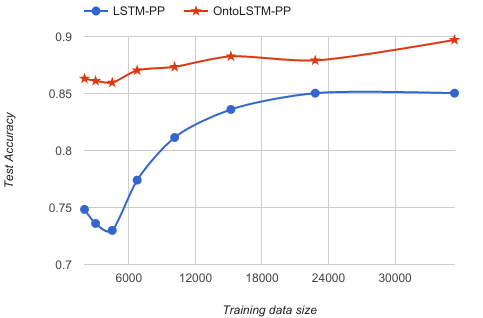
\includegraphics[width=3.6in]{figures/training_data_size.png}
\caption{Effect of training data size on test accuracies of OntoLSTM-PP and LSTM-PP.}
\label{fig:ontolstm_pp_data_size_variation}
\end{center}
\end{figure}

\begin{table}
    \centering
    \begin{tabular}{|l|c|}
    \hline
    \textbf{Model}	& \textbf{PPA Acc.}\\
    \hline
    full		& 89.7 \\
    - sense priors	& 88.4 \\
    - attention		& 87.5 \\
    \hline
    \end{tabular}
    \caption{Effect of removing sense priors and context sensitivity (attention) from the model.}
    \label{tab:ontolstm_pp_ablation_results}
\end{table}

\begin{figure*}
\begin{center}
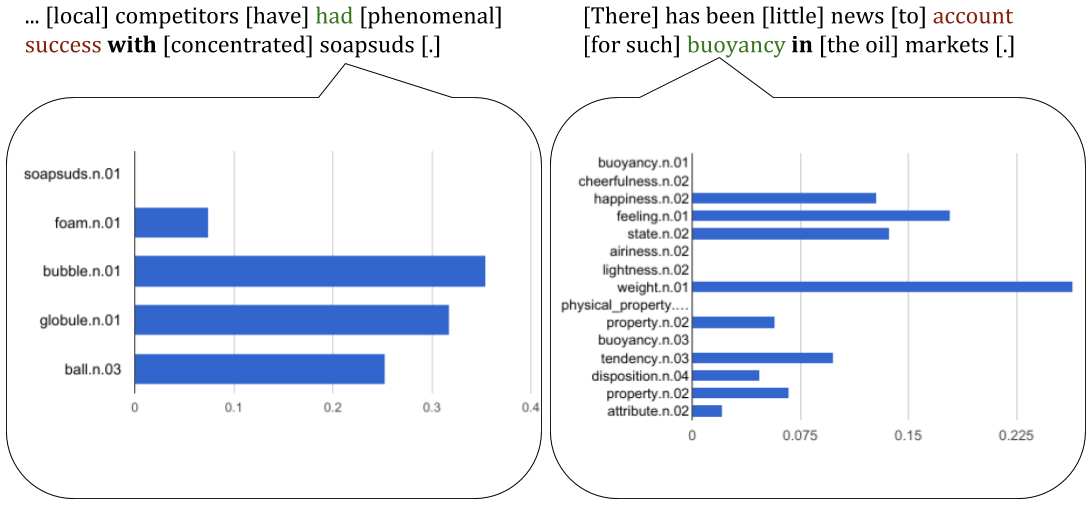
\includegraphics[width=6.2in]{figures/ontolstm_relative_attention.png}
\caption{Visualization of soft attention weights assigned by OntoLSTM to various synsets in Preposition Phrase Attachment}
\label{fig:ontolstm_pp_attention_visualization}
\end{center}
\end{figure*}
\paragraph{Qualitative analysis.} To better understand the effect of WordNet grounding, we took a sample of 100 sentences from the test set whose PP attachments were correctly predicted by OntoLSTM-PP but not by LSTM-PP. 
A common pattern observed was that those sentences contained words not seen frequently in the training data. Figure ~\ref{fig:ontolstm_pp_attention_visualization} shows two such cases where OntoLSTM-PP predicts the head correctly and
LSTM-PP does not, along with weights by OntoLSTM-PP to synsets that contribute to token representations of infrequent word types.
The prepositions are shown in bold, LSTM-PP's predictions in red and OntoLSTM-PP's predictions in green. Words that are not candidate heads or dependents are shown in brackets.
In both cases, the weights assigned by OntoLSTM-PP to infrequent words are also shown. The word types \textit{soapsuds} and \textit{buoyancy} 
do not occur in the training data, but OntoLSTM-PP was able to leverage the parameters learned for the synsets that contributed to their token representations.
Another important observation is that the word type \textit{buoyancy} has four senses in WordNet (we consider the first three), none of which is the metaphorical sense that is applicable to \textit{markets} as shown in the example here. Selecting a combination of relevant hypernyms from various senses may have helped OntoLSTM-PP make the right prediction. This shows the value of using hypernymy information from WordNet. Moreover, this indicates the strength of the hybrid nature of the model, that lets it augment ontological information with distributional information.

\paragraph{Parameter space.} We note that the vocabulary sizes in OntoLSTM-PP and LSTM-PP are comparable as the synset types are shared across word types. 
In our experiments with the full PP attachment dataset, we learned embeddings for 18k synset types with OntoLSTM-PP and 11k word types with LSTM-PP. Since the biggest contribution to the parameter space comes from the embedding layer,
the complexities of both the models are comparable.

\section{Textual Entailment}
\label{sec:ontolstm_snli}
We evaluate the capability of OntoLSTM to learn useful generalizations of concepts by testing it on
the task of textual entailment. We use the Stanford Natural Language Inference (SNLI) dataset \citep{bowman:15}.

\subsection{Data preprocessing} Since the dataset does not contain POS tag information unlike the PP attachment dataset,
we run Stanford's POS tagger \citep{toutanova:03} on the dataset.
To construct the tensor representation, we map the POS-tagged word to the first 
two synsets in WordNet (i.e. $S=2$), and extract the most direct five hypernyms 
(i.e., $H=5$). When a synset has multiple hypernym paths, we use the shortest 
one. In preliminary experiments, we found that using more word senses or more 
hypernyms per word sense does not improve the performance.
Like with the PPA dataset, words which do not appear in WordNet are assumed to
have one unique synset per word type with no hypernyms.

\subsection{Problem Definition}
Given a pair of sentences (premise and hypothesis), the model predicts one of 
three possible relationships between the two sentences: \textit{entailment}, 
\textit{contradiction} or \textit{neutral}.
We use the standard train, development and test splits of the SNLI corpus, which 
consists of 549K, 10K and 10K labeled sentence pairs, respectively.
For example, the following sentence pair is labeled \textit{entailment}:
 \begin{itemize}
  \item \textbf{Premise} \textit{Children and parents are splashing water at the 
pool.}
  \item \textbf{Hypothesis} \textit{Families are playing outside.}
 \end{itemize}
 
\subsection{Model Definition}
Following \cite{bowman2016fast}, our model for textual entailment uses two LSTMs with tied parameters
to  read the premise and the hypothesis of each example, then compute the vector $h$ 
which summarizes the sentence pair as the following concatenation (originally proposed by \cite{mou2015recognizing}):
$$h=\big[h_{\text{pre}}; h_{\text{hyp}}; h_{\text{pre}} 
-h_{\text{hyp}};h_{\text{pre}} *h_{\text{hyp}}\big]$$
where $h_\text{pre}$ is the output hidden layer at the end of the premise token 
sequence, $h_\text{hyp}$ is the output hidden layer at the end of the hypothesis 
token sequence.
The summary $h$ then feeds into two fully connected ReLU layers of size 1024, 
followed by a softmax layer of size 3 to predict the label.
The word embeddings and concept embeddings are of size 300, and the hidden 
layers 150.

The proposed model uses the WordNet grounded token embeddings, and we call it \textbf{OntoLSTM-TE}.
We compare it with two baselines: The first one is a simpler variant of \textit{OntoLSTM-TE}, and does not
use attention over synsets. We call it $\textbf{OntoLSTM-TE}_{\textbf{uni}}$. The second uses type level word representations, and 
we call it \textbf{LSTM-TE}.

The models are trained to maximize log-likelihood of correct labels in the 
training data, using ADAM \citep{kingma2014adam} with early stopping (up to 
twenty epochs).

\subsection{Experiments}
Table~\ref{tab:ontolstm_snli_results} shows the classification results. We also 
report previously published results of a similar neural architecture as an extra 
baseline: the 300-dimensional LSTM RNN encoder model in 
\cite{bowman2016fast}.\footnote{We note this is not the state of the art
on this dataset. This is the simplest sentence encoding based model for this task.}
They use GloVe as pretrained word embeddings while we jointly learn word/concept 
embeddings in the same model.
\cite{bowman2016fast}'s LSTM outperforms \textit{LSTM-TE} model by 0.9 absolute points 
on the test set. This may be due to the difference in input representations. 
Since we learn the synset representations in \textit{OntoLSTM-TE}, comparison with our LSTM 
implementations is more sensible.
The \textit{OntoLSTM-TE} outperforms \textit{LSTM-TE} by 1.4 absolute 
points on the test set, illustrating the utility of the ontology-aware word 
representations in a controlled experiment.

\begin{table}
    \centering
    \begin{tabular}{|l|c|c|c|}
    \hline
    \textbf{Model} & \textbf{GloVe} & \textbf{Train} & \textbf{Test}\\
    \hline
    LSTM-TE                        & No & 90.5 & 79.7 \\
    $\text{OntoLSTM-TE}_\text{uni}$  & No & 90.6 & 81.0 \\
    OntoLSTM-TE  & No & 90.5 & 81.1 \\ \hline
    LSTM (Bowman et al.) & Yes & 83.9 & 80.6 \\
    \hline
    \end{tabular}
    \caption{Results of OntoLSTM on the SNLI dataset}
    \label{tab:ontolstm_snli_results}
\end{table}


\subsection{Analysis}
\label{sec:ontolstm_snli_discussion}
\begin{figure}
\begin{center}
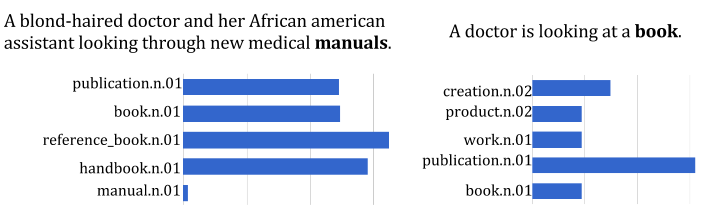
\includegraphics[width=5in]{figures/ontolstm_snli_comparison.png}
\caption{Visualization of soft attention weights assigned by OntoLSTM to various synsets in Textual Entailment}
\label{fig:ontolstm_snli_visualization}
\end{center}
\end{figure}

\paragraph{Generalization attention:} \label{sec:ontolstm_snli_generalization}
Fig.~\ref{fig:ontolstm_snli_visualization} shows one example from the test set of the 
SNLI dataset where hypernymy information is useful. 
The \textit{LSTM-TE} model shares no parameters between the lexical representations of 
\textit{book} and \textit{manuals}, and fails to predict the correct 
relationship (i.e., entailment). 
However, \textit{OntoLSTM-TE} leverages the fact that \textit{book} 
and \textit{manuals} share the common hypernyms \textit{book.n.01} and 
\textit{publication.n.01}, and assigns relatively high attention probabilities 
to these hypernyms, resulting in a similar lexical representation of the two 
words, and a correct prediction of this example.

The following is an example that \textit{LSTM-TE} gets right and \textit{OntoLSTM-TE} does not:
\begin{itemize}
 \item Premise: \textit{Women of India performing with blue streamers, in 
beautiful blue costumes.}
 \item Hypothesis: \textit{Indian women perform together in gorgeous costumes}
\end{itemize}
\textit{Indian} in the second sentence is an adjective, and \textit{India} in 
the first is an noun. By design, WordNet does not link words of different parts 
of speech. Moreover, the adjective hierarchies in WordNet are very shallow and 
\textit{gorgeous} and \textit{beautiful} belong to two different synsets, both 
without any hypernyms. Hence \textit{OntoLSTM-TE} could not use any generalization 
information in this problem.

\paragraph{Parameter space:} As mentioned earlier in the case of PP attachment problem,
the model size in \textit{LSTM-TE} and both variants of \textit{OntoLSTM-TE} are comparable
(11.1M and 12.7M parameters, respectively).

\section{Conclusion}
In this chapter, we showed a grounding of lexical items which acknowledges the semantic ambiguity 
of word types using WordNet and a method to learn a context-sensitive distribution over their representations.
We also showed how to integrate the proposed representation with recurrent neural networks for modeling sentences,
showing that the proposed WordNet-grounded context-sensitive token embeddings outperforms standard type-level embeddings
for predicting PP attachments and textual entailment.

We encoded a specific kind of background knowledge using WordNet in this work, but the methods described here can be extended 
to other kinds of structured knowledge sources as well. For example, one can effectively encode entities in text, using structured information
from Freebase. Such a model may help tasks like factual question answering.

One potential issue with the approach suggested in this chapter is
linking ambiguity. That is, deciding which entities in the background knowledge base, or concepts in the background ontology can be linked to
the tokens in the input utterance. In this chapter, we did not have to deal with this issue because linking words to WordNet concepts is a
trivial process. However, when extending this method to other kinds of knowledge bases, one may need to perform explicit entity or concept linking.